\documentclass{article}
\usepackage{tikz}
\usepackage{array}
\usepackage{calc}
\usepackage{setspace}
\usepackage{amsmath}
\usepackage{xspace}
\usepackage{color}
\usetikzlibrary{shapes.geometric, arrows}

\tikzstyle{startstop} = [rectangle, rounded corners, minimum width=3cm, minimum height=1cm,text centered, draw=black, fill=red!30]
\tikzstyle{io} = [trapezium, trapezium left angle=70, trapezium right angle=110, minimum width=3cm, minimum height=1cm, text centered, draw=black, fill=blue!30, text width = 2cm]
\tikzstyle{process} = [rectangle, minimum width=3cm, minimum height=1cm, text centered, draw=black, fill=orange!30, text width = 2cm]
\tikzstyle{decision} = [diamond, minimum width=3cm, minimum height=1cm, text centered, draw=black, fill=green!30, text width = 2cm]
\tikzstyle{arrow} = [thick,->,>=stealth]

\newcommand\mTW{1.25cm}
\newcommand{\citeme}{\textcolor{red}{[CITATION NEEDED]}\xspace}
\newcommand{\TODO}[1] {{\color{red}\textbf{TODO: #1}}}

\begin{document}
\title{XSGen}
\date{January, 25, 2017}
\author{Flanagan, Robert \and Scopatz, Anthony}
\maketitle
\onehalfspacing

\section{Introduction}


\section{XSGen Workflow}
The XSGen workflow is composed of three main parts as mentioned above \TODO{list again since in
a new section}. The first step is the simulation of the reactor core using a
Monte Carlo neutron transport simulation. The main result of this is the flux spectrum.
The spectrum is then collapsed with a a cross section database and converted into
a suite of one group cross sections for a reactor at a given time $t$ \TODO{units}
after the reactor has started up. These one group cross sections are then used inside of
a Bateman equation solve to calculate the burnup, neutron production, neutron destruction,
and transmutation matrices. The value of $t$ is set by the user when XSGen is executed.
The composition of the material at the end of the time step is then submitted back to
the Monte Carlo simulator as inpu. This process is repeated until the maximum time
step specified is reached. This flow is displayed in Figure \ref{fig:flow}.
\TODO{We need to mention OpenMC, PyNE, and Origen by this point since they are used
in the figure.}

\begin{figure}\center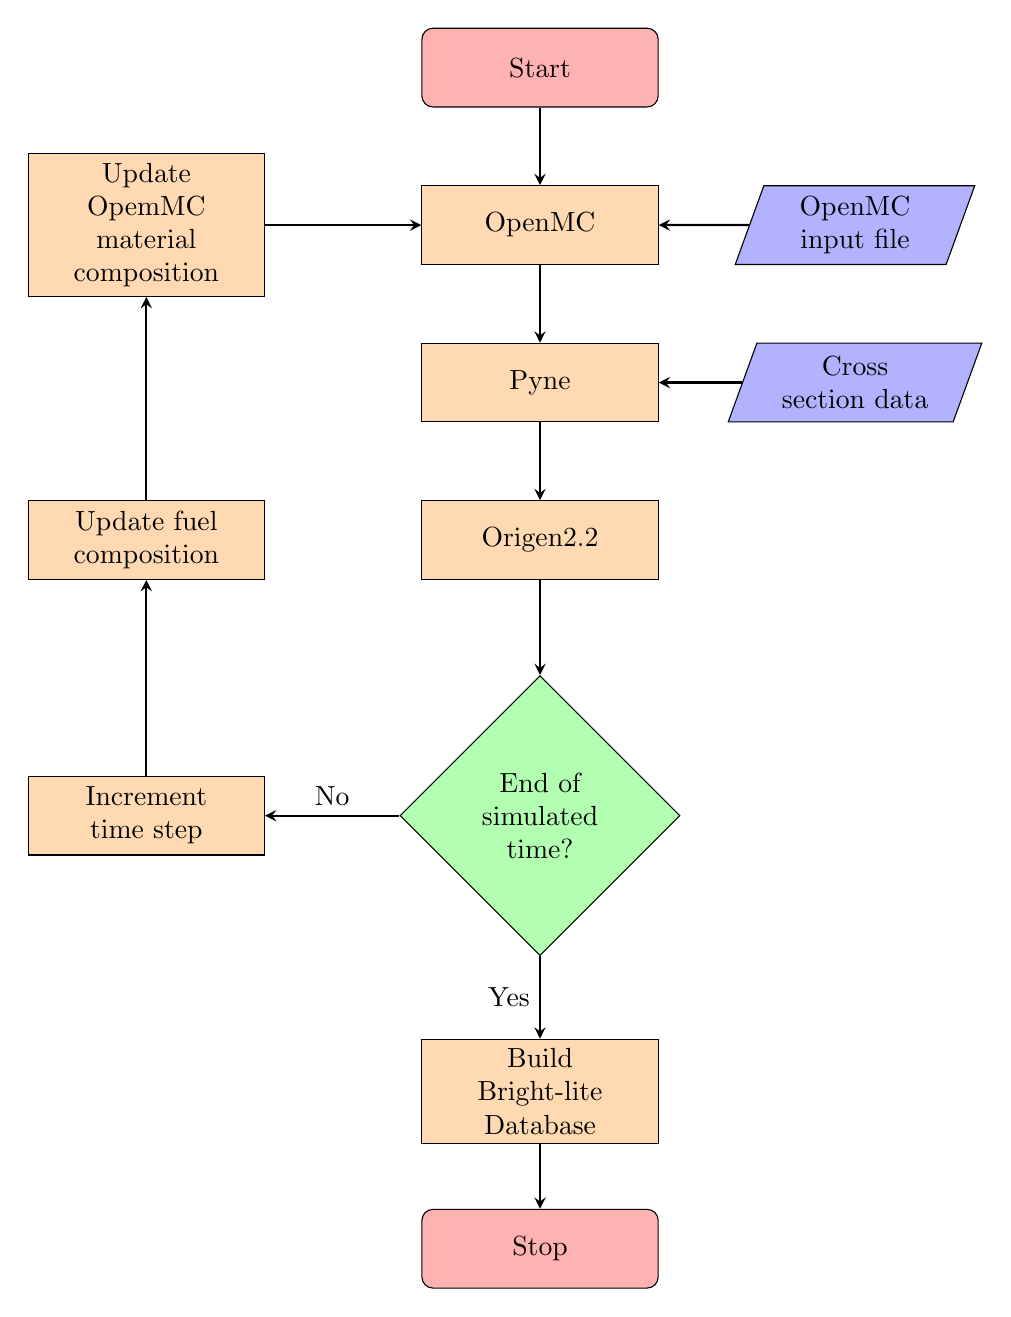
\begin{tikzpicture}[node distance=2cm]
\node (start) [startstop] {Start};
\node (openmc) [process, below of = start]{OpenMC};
\node (omcinput) [io, right of = openmc, xshift = 2cm]{OpenMC input file};
\node (omcupdate) [process, left of = openmc, xshift = -3cm]{Update OpemMC material composition};
\node (pyne) [process, below of = openmc]{Pyne};
\node (pynexs) [io, right of = pyne, xshift = 2cm]{Cross section data};
\node (origen22) [process, below of = pyne]{Origen2.2};
\node (compupdate) [process, left of = origen22, xshift = -3cm]{Update fuel composition};
\node (timecheck) [decision, below of = origen22, yshift = -1.5cm]{End of simulated time?};
\node (timeinc) [process, left of = timecheck, xshift = -3cm]{Increment time step};
\node (brightlite) [process, below of = timecheck, yshift = -1.5cm]{Build Bright-lite Database};
\node (stop) [startstop, below of = brightlite] {Stop};
\draw [arrow] (start) -- (openmc);
\draw [arrow] (omcinput) -- (openmc);
\draw [arrow] (omcupdate) -- (openmc);
\draw [arrow] (openmc) -- (pyne);
\draw [arrow] (pynexs) -- (pyne);
\draw [arrow] (pyne) -- (origen22);
\draw [arrow] (origen22) -- (timecheck);
\draw [arrow] (compupdate) -- (omcupdate);
\draw [arrow] (timeinc) -- (compupdate);
\draw [arrow] (timecheck) -- node[anchor=south]{No}(timeinc);
\draw [arrow] (timecheck) -- node[anchor=east]{Yes}(brightlite);
\draw [arrow] (brightlite) -- (stop);
\end{tikzpicture}
\caption{Flow chat of the XSgen process for building Bright-lite data tables.}
\label{fig:flow}
\end{figure}

\subsection{OpenMC}
OpenMC \citeme was used and the reference neutron transport software for modeling reactors.
OpenMC was chosen due to its availablity (it open source), ability to quickly perform
reactor oriented calculations, and the ability to compute scatering kernels.
Currently, XSGen only requires from the group fluxes from OpenMC.
Input templates for OpenMC can be specified in the XSGen run control file. Standard templates
may also be added to XSGen itself for use in future modeling.

\subsection{PyNE}
PyNE \citeme, a Nuclear Engineering toolkit library, is used to perform the group collapse
from cross section databases down to the one group or multigroup cross sections.
In the workflow here, PyNE is responsible for reading in cross section data from a wide
vareity of sources. It is able to synthesize cross section data - that may exist with
many different energy grids - down to a single energy group structure specified by the user.

The algorithm for collaspsing the cross sections, which PyNE performs in bulk, is as follows.
First, a partial energy matrix (PEM) is created. This matrix maps a higher resolution group
structures to lower resolution group structures. It does this by determining the contribution
of each of the higher resolution energy groups into the lower resolution energy groups using
a weighted sum. As this calculation can be computationally expensive it is only performed
once per time step. \TODO{Clarify: It is important to note that the dimensions of the PEM are set, and only
work the two group structures used to create it.}

Here, $\vec{\phi_h}$ represents the vector of group fluxes for $H$ energy groups with
a group structured defined by $E_H$ bin boundaries. Likewise, $\vec{\phi_g}$ represents
the collapsed flux with $G$ groups and $E_G$ bin boundaries. The partial energy
matrix is then defined by the relations below,

\TODO{PEM CALCULATION}

For the current use case of Bright-lite, this lower group structure is always a one group.
However, XSGen mayu generate any energy group structure desired.
Thus shifting a given group structure into a desired one using the PEM is simply a matter
of taking the dot product of the PEM by the original group structure.

\[ \vec{\phi_g} = P \cdot \vec{\phi_h} \]

Additionally, group-wise cross sections for each isotope must be calculated. This is done using the raw pointwise cross section data through the following method.

$$\sigma_{i,g}^x = \frac{\sum_{E_j=E_l}^{E_j=E_u}0.5*[\sigma(E_j)+\sigma(E_{j+1})]*[E_{j+1}-E_{j}]}{E_u-E_l}$$

Here $E_l$ and $E_u$ represent the lower and upper bounds of the energy group, $E_j$ represents the energy of a pointwise cross section in the data set, $\sigma(E_j)$ represents the cross section at energy $E_j$, and $\sigma_{i,g}^x$ represents a group wise cross section for isotope x, and cross section i.

With the one group flux, and group-wise cross sections, it is possible to generate the one group, flux weighted, cross sections using the following equation.

$$\sigma_{i}^x=\frac{[PEM∙(\sigma_{i,g}^x*\phi)]}{\sigma_g}$$

Here $\sigma_{i}^x$ represents the one group cross section of specific type i, for isotope x. This process is repeated for all isotopes and cross section, and those values are input into an Origin 2.2 TAPE9 file.

Pyne will also allow the user to incorperate the effects of self-shielding into XSgen. It does this build building an energy dependent function of weights of each isotope. These weights scale the one group cross section depending on the density of the isotope represented by this cross section. The more delute a isotope is within a material composition, the lower the effective cross section of the isotope. This done using the following equation.

$$\omega_{y,n}=\frac{1}{\frac{\sum_{x\neq y}N^x * \sigma_{t,g}^x}{N^y}+\sigma_{t,g}^y}$$

Here all isotopes in the fuel are included in the set of X, and Y is the isotope in question. $N_y$ represents the number density of isotope Y, and $\sigma_{t,n}^x$ represents a flux weighted total cross section of an isotope, x, in a specific energy bin, n.

Therefore similar to the mechanism described in the previous equation for calculated the one group flux weighted cross sections, these are multigroup flux weighted cross sections. Because this data is pointwise, a pointwise flux is also required. OpenMC will not output a point wise flux, so a fundamental pointwise flux is used as a supplement. The equation for this flux is as follows.

\large

\[ \phi = \begin{cases}
      \frac{2*\pi*\sqrt{E*1e6}*e^{\frac{-E*1e6}{kT}}}{(\pi*kT)^1.5} & E\leq 0.155e-6 \\
      \frac{1}{\sqrt{2E*1e6}} + 0.453e^{-1.036E}*\sinh{\sqrt{2.29E}} & E > 0.155e-6 \\
   \end{cases}
\]

Where $k$ is the Boltzman constant, $T$ is the temperature, and E is the energy. This formulation of the flux can be shown visually in Figure \ref{fig:therm}.
\begin{figure}[h]
  \center
  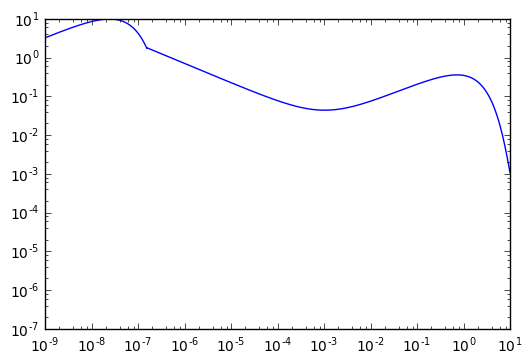
\includegraphics[scale=0.8]{thermspec.png}
  \caption{The effects of self-shielding on the cross sections for Uranium 235.}
  \label{fig:therm}
\end{figure}

The end result of all of this is a two-dimensional matrix of X (number of isotopes) by G (number of groups). The number in each entry of the matrix is the cross section weight for a specific isotope, in a specific energy group. These weights must be recalculated every time-step as the number densities of the isotopes in the fuel will charge as burnup increases.

Note, that the pointwise cross sections used in these calculation must be provided by an outside source. PyNE is capable of reading in cross sections from several different cross section libraries including; ENDF, Cinder, EAF, and OpenMC. In this case the OpenMC cross sections were used.

The effects of self shielding on U235 inside of a fuel pellet can be seen in Figure \ref{fig:index}.
\begin{figure}[h]
  \center
  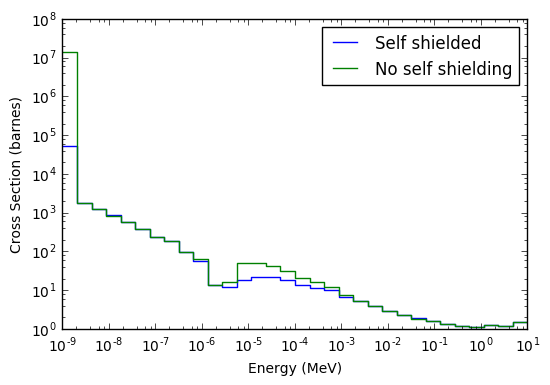
\includegraphics[scale=0.8]{index.png}
  \caption{The effects of self-shielding on the fission cross section of Uranium 235 inside a fuel pellet.}
  \label{fig:index}
\end{figure}

\subsection{Origin2.2}
Once the TAPE9 has been constructed it is used to perform two types of burnup operations. The first burnup is performed on the fuel. This includes the full list of isotopes currently in the fuel. Once this burnup is performed the isotopic vector at the end of the fuel burn is passed back to OpenMC to start the operation all over again.

The second type of burnup calculation is used to build a dataset for a specific isotope. These burnup runs take one kilogram of a pure isotope as the input fuel. At the end of the run, the burnup, neutron production/destruction, and transmutation matrix are all recorded. The isotopes of interest are chosen ahead of time by the user of the software, typically these are the isotopes that the user wishes to use as the input fuel for the reactor type/design that they are investigating.

\section{XSGen Results}

\section{Benchmarking}
\subsection{LWR Test Cases}
XSGen by itself can not directly be tested against operating reactor systems. It was originally designed to produce datasets a medium fidelity reactor model known as Bright-lite. Therefore, to benchmark XSGen it will be used in conjunction with Bright-lite to produce burnups and isotopes for several known reactor systems.  As Bright-lite has already been benchmarked several times using other datasets [BRIGHT-LITE Benchmark Citations] it is assumed that the operations within Bright-lite are accurate and any deviations within the results come from XSGen.

The most well studied reactors in the world are light water reactors and as such these will be used as benchmarking tools for XSGen. Primarily the cases represent a range of different enrichments in several light water reactors, comparing the results from XSGen/Bright-lite to recipes from VISION. Additionally, the values will be tested against two cases modelling reactor startup behavior.  [vision citation / transition citation].

The XSGen/Bright-light will be benchmarked against VISION at 3.0, 3.5, 4.0, and 4.5 percent enrichment. Three batch cores will be assumed for all the enrichment test cases.
The two cases being used to test XSGen in startup behavior will be a 3.1$\%$ enriched light water reactor using four batches and a 3.6$\%$ enriched light water reactor using four batches. The cases will be compared using burnups, isotopic composition of fresh and used fuel.

\subsection{Results}

\begin{table}[!htb]
\centering
\small
\caption{A comparison of the output isotopics at equalibrium in the VISION fuel cycle simulator and the XSGen-Bright-lite system.}
\label{tab:a}
\vspace{0.5em}
\hspace*{-5em}\begin{tabular}{|c| m{\mTW} m{\mTW} m{1cm}| m{\mTW} m{\mTW} m{1cm} | m{\mTW} m{\mTW} m{1cm} |}
 & \multicolumn{3}{c}{3.0\%} & \multicolumn{3}{c}{3.5\%} & \multicolumn{3}{c}{4.0\%} \\
Isotope & VISION & XSGen & Diff & VISION & XSGen & Diff & VISION & XSGen & Diff \\
\hline
U235 & 6.75E-3 & 6.70E-3 & -0.78 & 6.80E-3 & 6.71E-3 & -1.30 & 6.95E-3 & 6.91E-3 & -0.562 \\
Pu238 & 1.23E-4 & 1.27E-4 & 3.01 & 1.85E-4 & 1.86E-4 & -0.41 & 2.52E-4 & 2.55E-4 & 1.35 \\
Pu239 & 5.15E-3 & 5.25E-3 & 1.95 & 5.41E-3 & 5.45E-3 & 0.66 & 5.64E-3 & 5.67E-3 & 0.57 \\
Pu240 & 2.38E-3 & 2.40E-3 & 0.97 & 2.60E-3 & 2.61E-3 & 0.25 & 2.78E-3 & 2.79E-3 & 0.4 \\
Pu241 & 1.30E-3 & 1.35E-3 & 3.69 & 1.48E-3 & 1.52E-3 & 2.74 & 1.62E-3 & 1.62E-3 & -0.02 \\
Pu242 & 5.43E-4 & 5.48E-4 & 0.88 & 6.92E-4 & 6.93E-4 & 0.10 & 8.17E-4 & 8.19E-4 & -0.28 \\
Am241 & 3.56E-5 & 3.86E-5 & 8.81 & 4.59E-5 & 5.17E-5 & 12.60 & 5.55E-5 & 6.04E-5 & 8.79 \\
Am243 & 9.38E-5 & 9.01E-5 & -3.94 & 1.37E-4 & 1.26E-4 & -7.47 & 1.76E-4 & 1.74E-4 & -1.40 \\
Cm242 & 1.38E-5 & 1.34E-5 & -3.19 & 1.88E-5 & 1.79E-5 & -4.91 & 2.33E-5 & 2.31E-5 & -0.83 \\
Cm244 & 2.79E-5 & 2.57E-5 & -7.94 & 4.38E-5 & 4.54E-5 & -6.06 & 7.06E-5 & 7.00E-5 & -0.90 \\
\hline
\end{tabular}
\end{table}

Table \ref{tab:a} shows a very strong agreement between VISION and Bright-light results using datasets created from light water reactors designed to these particular enrichments. Bright-light has been benchmarked [Bright-lite citations] against VISION previously using other datasets. This shows that given XSGen generated datasets allows for Bright-lite to match VISION to a 5\% tolence for a majority of isotopes. Those that exhibit the greatest deviations are high order transuranics.

Am241 shows the largest deviations from the VISION data. There is more Am241 in every case than expected by the VISION results, and less of the species that are arise due to the presence of Am241; Am243, Cm242, Cm244. These results can be explained by a neutron absorption cross section error in Am241. If the neutron absorption cross section for Am241 is too low it can never transmute into Am242 and Am243, which in turn leads to an absence of curium isotopes.

\begin{table}[!htb]
\centering
\caption{NEA core discharge data for a 3.1\% enriched light water reactor with startup behavior.}
\label{tab:b}
\begin{tabular}{lllll}
Batch & Burnup (MWd/kg) & U235 (\%) & Fissile Pu (\%) & Total Pu(\%) \\
1 & 12.04 & 0.64 & 0.464 & 0.633 \\
2 & 23.86 & 0.76 & 0.6 & 0.818 \\
3 & 31.75 & 0.8 & 0.677 & 0.921 \\
4 & 32.00 & 0.85 & 0.697 & 0.943 \\
Equil. & 33.00 & 0.85 & 0.688 & 0.943
\end{tabular}
\end{table}

\begin{table}[!htb]
\centering
\caption{The startup values and percent difference from the NEA data for the XSGen/Bright-lite reactor system.}
\label{tab:c}
\begin{tabular}{lllllllll}
 & \multicolumn{2}{l}{Burnup (MWd/kgIHM)} & \multicolumn{2}{l}{U235 (\%)} & \multicolumn{2}{l}{Fissile Pu (\%)} & \multicolumn{2}{l}{Total Pu (\%)} \\
Batch & Value & \%Diff & Value & \%Diff & Value & \%Diff & Value & \%Diff \\
1 & 13.570 & 12.754 & 0.656 & 2.50 & 0.550 & 18.737 & 0.680 & 7.541 \\
2 & 22.040 & -7.628 & 0.723 & -4.868 & 0.641 & 6.919 & 0.835 & 2.189 \\
3 & 32.510 & 2.394 & 0.789 & -1.375 & 0.710 & 4.883 & 0.970 & 5.231 \\
4 & 31.230 & -2.406 & 0.851 & 0.117 & 0.680 & -2.254 & 0.906 & -5.031 \\
5 & 33.010 & 0.030 & 0.843 & -0.824 & 0.703 & 2.198 & 0.946 & 0.285 \\
Equal. & 33.020 & 0.060 & 0.855 & 0.588 & 0.700 & 1.833 & 0.951 & 0.820
\end{tabular}
\end{table}

Table \ref{tab:b} shows how XSGen/Bright-lite compares to the NEA results. The equilibrium results here show good agreement with this case. As Bright-lite is often used to derive output isotopics from used fuels to be passed onto recycle scenarios, accurately predicting the equilibrium output isotopics is important.

The results of the start up isotopics can be seen in Table \ref{tab:c}. There are some discrepencies in these results. First, the amount of plutonium generated within the first batch is significantly higher within Bright-lite compared to the NEA data. This trend only continues for the first two cycles. Due to the way Bright-lite operates, this is caused by the lower enriched batches within the startup core that do not have neutron poisons from fission products or other actinides. This means that there is a higher effective flux striking a high amount of U238 causing more generation of Pu239. The NEA benchmark has these low enrichment startup batches spread more evenly, Bright-lite has them all inside the inner most part of the circle.

\begin{table}[!htb]
\centering
\caption{NEA data for a 3.6\% enriched light water reactor start up behavior.}
\label{tab:d}
\begin{tabular}{lllll}
Batch & Burnup (MWd/kg) & U235 (\%) & Fissile Pu (\%) & Total Pu(\%) \\
1 & 13.9 & 0.840 & 0.474 & 0.629 \\
2 & 22.67 & 0.721 & 0.642 & 0.892 \\
3 & 32.36 & 0.647 & 0.716 & 1.039 \\
4 & 41.00 & 0.640 & 0.785 & 1.177 \\
5 & 39.00 & 0.940 & 0.808 & 1.166 \\
6 & 40.60 & 0.88 & 0.817 & 1.194 \\
Equil. & 42.50 & 0.81 & 0..827 & 1.223
\end{tabular}
\end{table}

\begin{table}[!htb]
\centering
\caption{XSGen / Bright-lite data for the 3.6\% enriched light water reactor start up behavior.}
\label{tab:e}
\begin{tabular}{lllllllll}
 & \multicolumn{2}{l}{Burnup (MWd/kgIHM)} & \multicolumn{2}{l}{U235 (\%)} & \multicolumn{2}{l}{Fissile Pu (\%)} & \multicolumn{2}{l}{Total Pu (\%)} \\
Batch & Value & \%Diff & Value & \%Diff & Value & \%Diff & Value & \%Diff \\
1 & 13.37 & -3.84 & 0.930 & 10.77 & 0.62 & 30.43 & 0.78 & 23.53 \\
2 & 22.69 & 0.07 & 0.82 & 13.02 & 0.72 & 12.81 & 0.96 & 7.49 \\
3 & 32.38 & 0.03 & 0.72 & 11.08 & 0.78 & 8.46 & 1.07 & 2.69 \\
4 & 42.57 & 3.83 & 0.61 & -5.33 & 0.804 & 2.42 & 1.14 & -2.94 \\
5 & 41.00 & 5.13 & 0.85 & 9.526 & 0.79 & -2.81 & 1.10 & -5.91 \\
6 & 43.83 & 3.04 & 0.82 & 6.53 & 0.79 & -3.58 & 1.11 & -7.45 \\
Equal. & 42.32 & -0.43 & 0.81 & -0.44 & 0.79 & -4.54 & 1.11 & -9.42
\end{tabular}
\end{table}

Table \ref{tab:d} and Table \ref{tab:e} are repeats of Table \ref{tab:b} and Table \ref{tab:c} for the 3.6$\%$ enriched light water reactor. Again, you see a similar trend in these two with the exception that the equilibrium results for the total amount of plutonium within the reactor is 9.2$\%$ lower in the Bright-lite model. The amount of fissile plutonium is also lower, but within acceptable bounds. The lower amount of fissile plutonium leads to less transmutations into the high order actinides.

\section{MOX Case}
Simply replicating the behavior of a light water reactor would not show off the full capabilities of the XSGen software. To demonstrate the capability of the system to extend to more advanced reactor types, XSGen will be used to generate a MOX fuel library for Bright-lite. It will then be used to simulate a single pass MOX reactor. In order to compare this on an apples to apples basis, the input fuel into the Bright-lite reactor will be exactly the same as that for a similar VISION reactor. This test will be able to demonstrate the flexibility of the combined XSGen/Bright-lite system that allows it to model advanced reactor types.

\begin{table}[!htb]
\centering
\caption{Comparison of VISION and Bright-lite result from a single pass MOX reactor.}
\label{tab:g}
\begin{tabular}{llllll}
Isotope & Input Composition & Vision & Bright-lite & Difference(\%) \\
U234 & 2.20E-4 & 2.11E-4 & 2.00E-4 & -5.0\\
U235 & 7.08E-3 & 4.05E-3 & 4.00E-3 & -1.2\\
U236 & 5.28E-3 & 4.97E-3 & 5.60E-3 & 12.6\\
U238 & 8.80E-1 & 8.51E-1 & 8.62E-1 & 1.3\\
Pu238 & 2.85E-3 & 3.22E-3 & 3.01E-3 & -6.5\\
Pu239 & 5.66E-2 & 3.31E-2 & 3.15E-2 & -4.6\\
Pu240 & 2.70E-2 & 2.42E-2 & 2.54E-2 & 5.0\\
Pu241 & 1.17E-2 & 1.31E-2 & 1.27E-2 & -3.3\\
Pu242 & 8.00E-3 & 8.90E-3 & 8.68E-3 & -2.6\\
Am241 & 1.18E-3 & 1.72E-3 & 1.60E-3 & -7.2\\
Am243 & - & 1.96E-3 & 1.83E-3 & -6.6\\
Cm242 & - & 2.62E-4 & 2.46E-4 & -6.4\\
CM244 & - & 1.03E-3 & 9.84E-4 & -4.4
\end{tabular}
\end{table}

The data in Table \ref{tab:g} shows that the results of Bright-lite given the new XSGen MOX reactor cross section fairs quite well compared to VISION. There are some outliers in the behaviors, specifically the higher order species and U236. The issues with the higher order actinides, Am241 and higher, most likely stem from the high amount of Pu240. This suggest that Pu240 is not transmuting into Pu241 at a high enough rate, which therefore lowers the equalibrium concentration of Pu241 and all isotopes that derive from it.

One of the possible primary causes of this is uncertainity in the exact dimensions and behavior of the VISION MOX reactor. In order to get the most accurate results XSGen needs to know the specification of the MOX reactor. Instead for this work a generic 17x17 light water reactor core was chosen to use as a base for the XSGen run. If the input and output compositions generated for VISION were made from a reactor core of a different design it would result in slightly different cross sections and therefore different behavior.

\section{Conclusion}


\end{document}

